% 项目导读（中文）：面向完全未接触过本项目的读者；数字与正式报告一致。
% 编译（LM2，两遍，目录 docs/report/stage_report_1/）：export PATH=/data6/jinxinhao/texlive/2026/bin/x86_64-linux:$PATH
%   xelatex summary_plain_zh.tex && xelatex summary_plain_zh.tex
\documentclass[11pt]{article}
\usepackage[margin=1in]{geometry}
\usepackage{amsmath,amssymb}
\usepackage{booktabs}
\usepackage{graphicx}
\usepackage{xcolor}
\usepackage{xeCJK}
\setCJKmainfont{FandolSong-Regular}[
  Extension = .otf, BoldFont = FandolSong-Bold,
  AutoFakeBold = 2.2, AutoFakeSlant = 0.2]
\setCJKsansfont{FandolHei-Regular}[Extension = .otf, AutoFakeBold = 2.2]
\renewcommand{\figurename}{图}
\usepackage[hidelinks]{hyperref}
\emergencystretch=3em

\title{\bfseries AI 看病理切片，为什么“看不见”将死的细胞？\\[6pt]
\large ——阶段报告一导读（课程项目 bdd26）}
\author{}
\date{2026 年 9 月 28 日}

\begin{document}
\maketitle

\begin{quote}
\textbf{一句话总结}：我们研究了 AI 在显微镜图像里找细胞核、认细胞类型的能力，为一个公认
的长期短板找到了贯穿所有实验的解释——不是“认错”，而是“看不见”；试了五种补救方法，在事
先约定的判定标准下都无效；还发现一种新式“考试”方法会把模型的真实排名几乎完全考反。
\end{quote}

\section*{背景：让 AI 帮医生看切片}

医生诊断肿瘤，经常要在显微镜下看染色的组织切片，逐个找出细胞核并判断它是哪一种细胞。这
件事费时费力，于是研究者训练 AI 来做：给它一张 40 倍放大的数字切片照片，它要把每个细胞
核的轮廓勾出来，并说出它属于哪一类。

为了比较 AI 的好坏，学界有一份公开的“标准考卷”——PanNuke 数据集：约 20 万个人工标注的
细胞核，来自 19 种人体组织，分成五大类（肿瘤细胞、炎症细胞、结缔组织细胞、非肿瘤的上皮
细胞，以及一类特殊的“凋亡核”——细胞死亡后留下的皱缩、碎裂、深染的残迹）。凋亡核值得单
独关注：有效的抗癌治疗往往伴随大量细胞死亡，凋亡核的多少对判断肿瘤状态和疗效有参考价值。

考卷按 0 到 1 打分。这个分数同时要求“找得准”（轮廓对得上）和“认得对”（类型不判错），
两项都好才能得高分。

\section*{发现一：换更强的模型几乎不涨分，但有一类细胞谁都认不好}

近五年新模型层出不穷，整个领域在这份考卷上的最好成绩也只从约 0.46 提高到 0.51——而后文
会看到，光评测配方里的“水分”就可能值 2 个百分点，真正的进步比排行榜显示的还要小。更扎
眼的是凋亡核：近五年所有已发表模型在这一类上的得分都卡在 0.13--0.18，而其它类型的细胞核
一般在 0.4 以上。

\section*{发现二：问题不是“认错”，而是根本“看不见”}

我们把复现模型的错误逐个拆开（用通行判定标准：预测轮廓与人工标注重叠过半才算检出）：
38.5\% 的凋亡核，模型给出的答案里根本没有它——不是把它认成了别的类型，而是压根没把它当
成细胞；作为对比，其它类型完全漏检的只有 8--15\%（图~\ref{fig:zhdecomp}）。

\begin{figure}[ht]
\centering
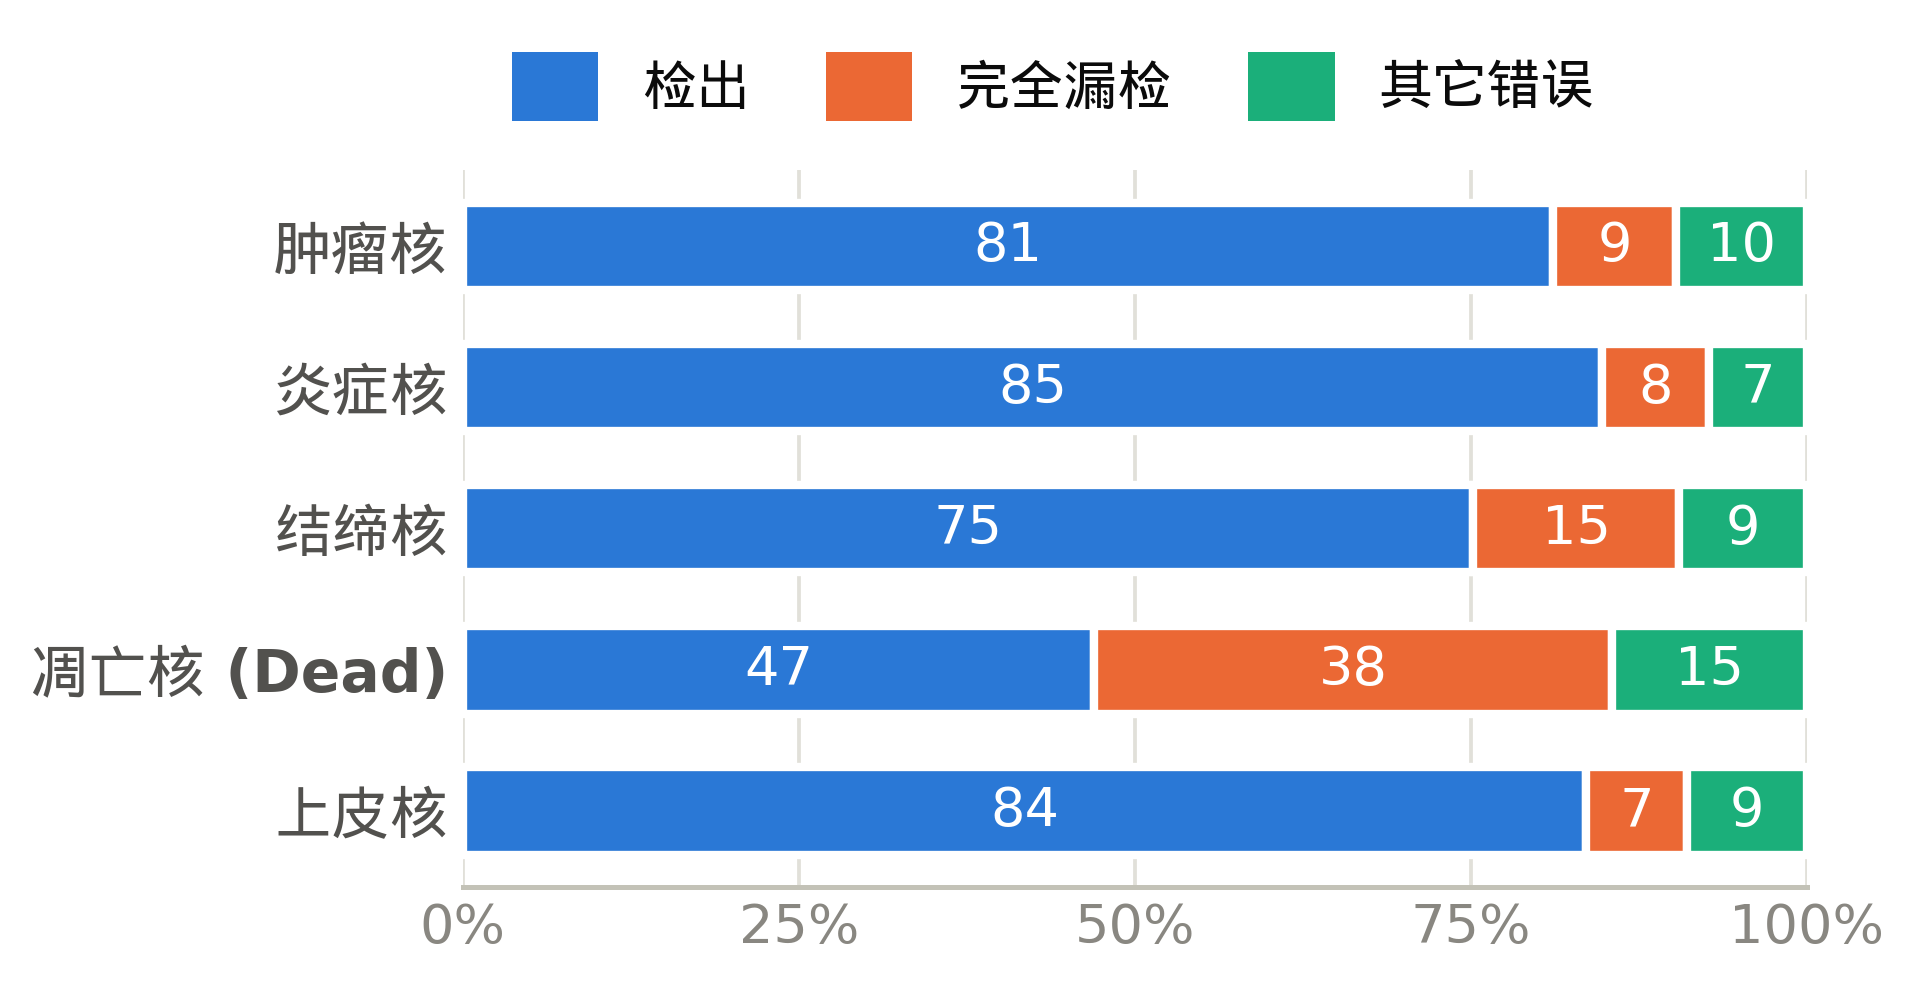
\includegraphics[width=0.95\linewidth]{figs/chart_decomp_zh.png}
\caption{五类细胞核的错误分解（CellViT-UNI，折 3）。蓝色“检出”指预测轮廓与人工标注重叠
过半；橙色“完全漏检”指模型答案里根本没有这个核。凋亡核（Dead）一行有 38\% 完全漏检，
是其它类的 3--5 倍。}
\label{fig:zhdecomp}
\end{figure}

更有意思的是，我们直接到漏检位置的图像区域去读模型两个部件的输出：负责“找细胞”的部件几
乎全静默（平均概率只有 0.16，仅在 17\% 的核里有反应），而负责“辨类型”的部件却给出约
26\% 的凋亡概率（其它类型只有约 1\%）。一句话，\textbf{问题出在“眼睛”（检测），不在
“脑子”（分类）}。顺带一提，检出来的凋亡核里也有约三成类型判错、约一成被并进旁边核的轮
廓——所以就算不算漏检，分数也上不去。

\begin{figure}[ht]
\centering
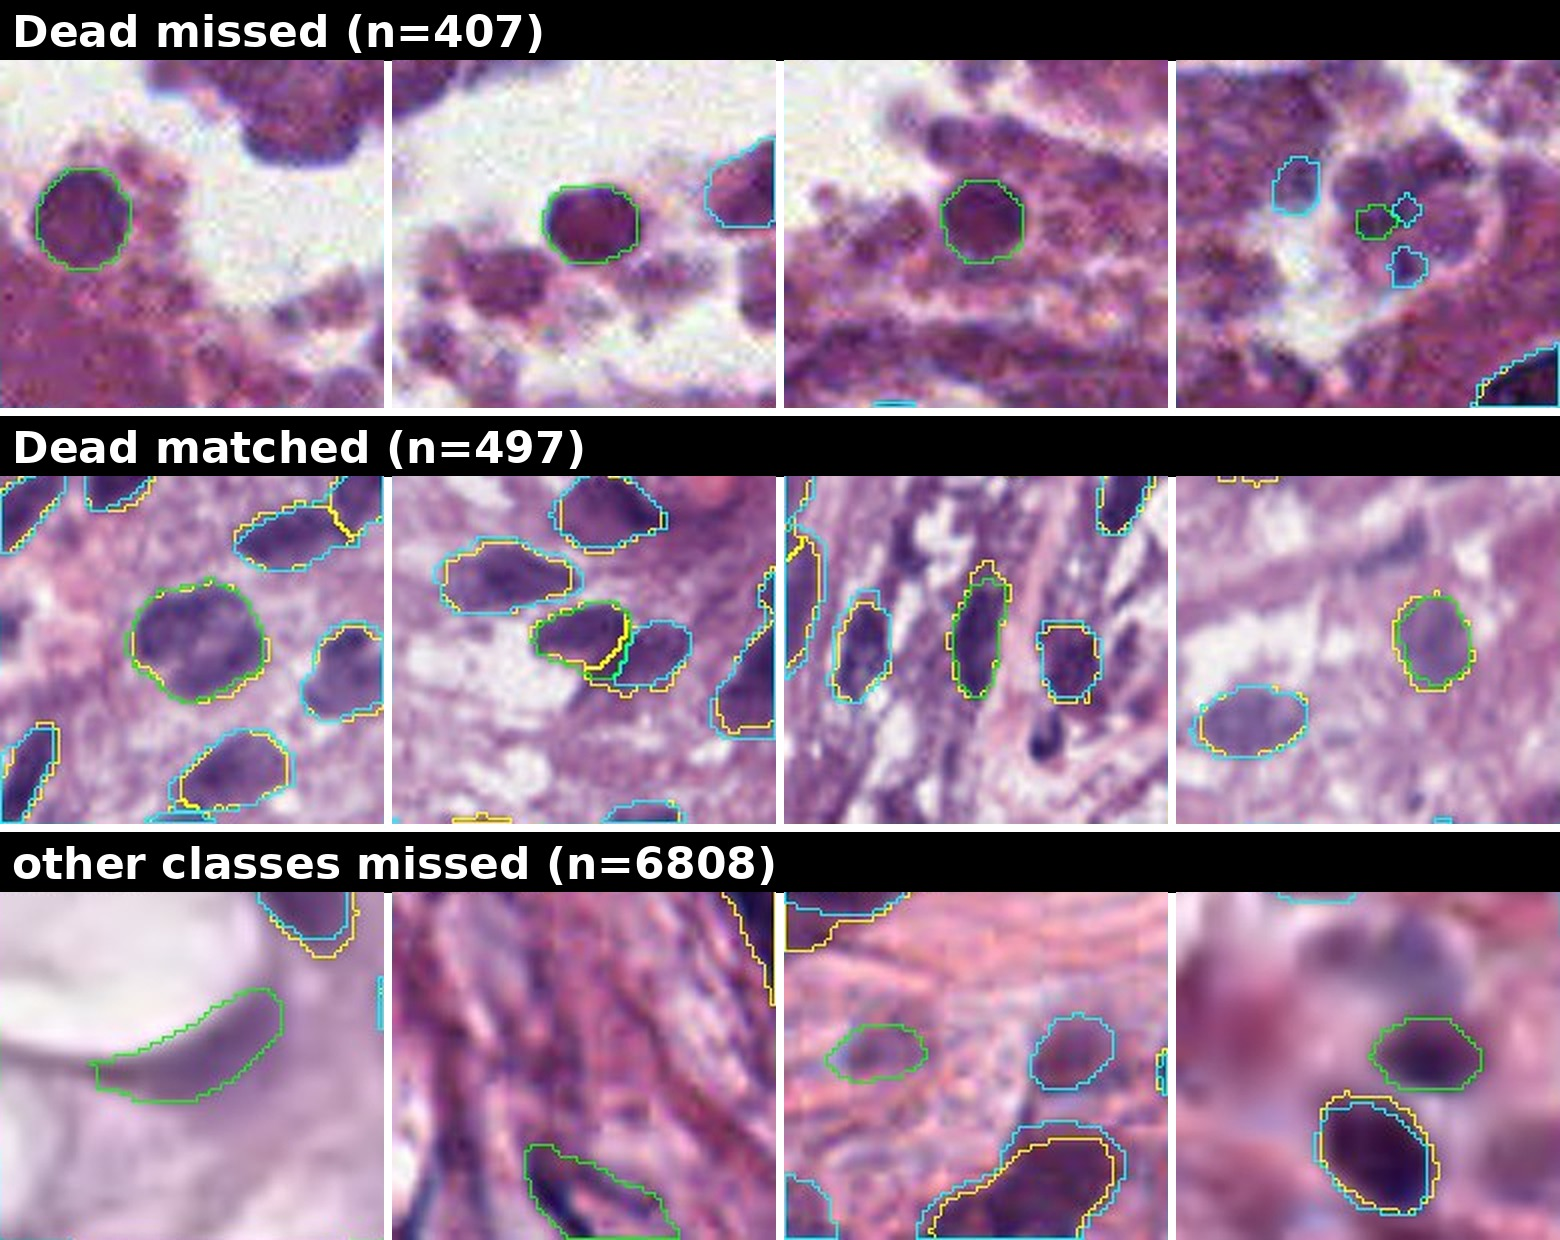
\includegraphics[width=0.86\linewidth]{figs/dead_missed.jpg}
\caption{模型找核的示例（CellViT-UNI，折 3；每组 4 个视野）：绿色是人工标注的目标核，
黄色是模型画出的核，青色是图中其它标注。上排“Dead missed”：凋亡核的绿色轮廓没有任何
黄框对应——模型完全没看见它们（407 个）；中排“Dead matched”：被正常检出的凋亡核
（绿黄重合）；下排“other classes missed”：其它类型漏检的对照——漏检率只有凋亡核的
约 1/3 到 1/5。}
\label{fig:deadmissed}
\end{figure}

\section*{发现三：五种补救办法，在事先约定的标准下全部无效}

\begin{enumerate}
\item 请病理“图文大模型”（见过大量病理图片和医学文字描述的 AI）帮忙重新判型——无效。
      这一条与下一条是最先试的：当时以为问题出在“认错类型”上，正是它们的失败促使我们去
      数漏检；
\item 在模型输出的概率图上调整判定门槛、翻找被埋没的小块，把漏掉的核“捞回来”——无效；
\item 训练时给凋亡核和“小核”加大权重（凋亡核的个头往往只有普通核的约三分之一）——无效；
\item 把真实的凋亡核“复制粘贴”进训练图的空白处——不仅无效，反而让凋亡核分得更差：模型
      把“空白处冒出的小核”当成了凋亡的标志，反而搞乱了类型边界；
\item 用图像生成 AI 照着标注“凭空画”新的训练图——无效。这条路先暴露了一个更根本的问题：
      生成器只接收“在这个位置画一个核”的指令，并不真正知道哪个核该是凋亡核，结果它画出来
      的孤立小核全都长得像普通淋巴核——七百多个生成的核里，能被认出是凋亡核的数量是零。
      若强行给这些“不像凋亡”的核打上凋亡标签，就又落回第 4 种方法的坑（标签与外观不符）。
      退而求其次、按生成图的实际长相来标注再训练，整体分数仍停在噪声范围内，凋亡核的变化
      也在噪声边缘——因为合成图能补的只是“多见些小核”，补不了真正缺的“在真实切片里看见
      凋亡核”的能力。
\end{enumerate}

这些失败不是白做。每种方法都在 3 个随机种子上重复训练、事先写明“怎样才算成功”，小于噪
声的差异一律不算数（同一模型换个随机种子重训，整体分自己就会波动约 $\pm$0.2 个百分点，
凋亡核甚至会波动约 $\pm$0.7 个百分点）。小核本来就难检出——各类皆然；但凋亡核即使个头
不小也常被漏掉（大个头凋亡核的漏检率是其它大核的 6 倍），说明还有“长得不像核”的外观问
题：很多凋亡核只是淡染的碎屑，没有深色的核。这些证据共同指向一个结论：缺陷很可能出在模
型的底层架构上，换数据、换训练技巧都救不了。

而且，当我们把模型拿到一套公开的黑色素瘤（一种皮肤癌）数据上考试，其它类型的细胞仍能正
常检出，唯独凋亡核的成绩几乎归零（图~\ref{fig:zhpuma}）——这个短板会跟着模型走。（也要
说明：凋亡核的人工标注本身就有少量模糊之处，这一类天然难上加难。）

\begin{figure}[ht]
\centering
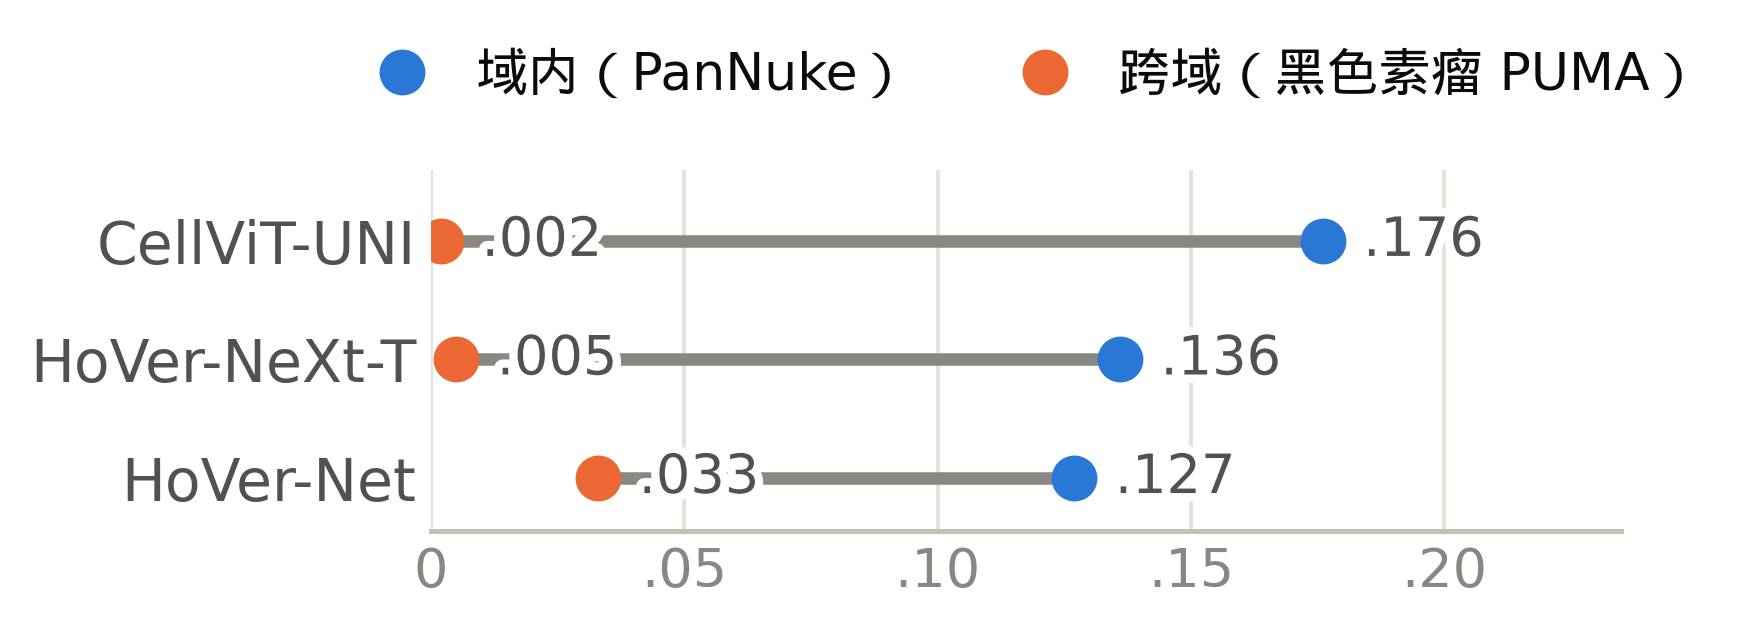
\includegraphics[width=0.82\linewidth]{figs/chart_dead_puma_zh.png}
\caption{三种模型的凋亡核（Dead）得分：域内考试（PanNuke）vs.\ 跨域考试（黑色素瘤数据
PUMA）。跨域时所有模型的凋亡核得分都跌到接近 0。}
\label{fig:zhpuma}
\end{figure}

\section*{发现四：一种新式“考试”会把模型的真实水平考反}

我们还尝试了一种流行的新思路：用生成式 AI 把考卷图片重新“画”一遍——每个细胞的位置和标
准答案都不变，只改变画面外观（比如背景换成别的组织、染色换成别家的）。本意是模拟“模型
到了新医院、新病种的数据上还靠不靠谱”。结果发现，\textbf{这种“换皮不换芯”的考试会把排
名考反（几乎正好颠倒）}：在真实跨病种测试（就是上面那套黑色素瘤等外部数据）中最稳的模
型，在这种考试里反而显得最脆弱。

\begin{figure}[ht]
\centering
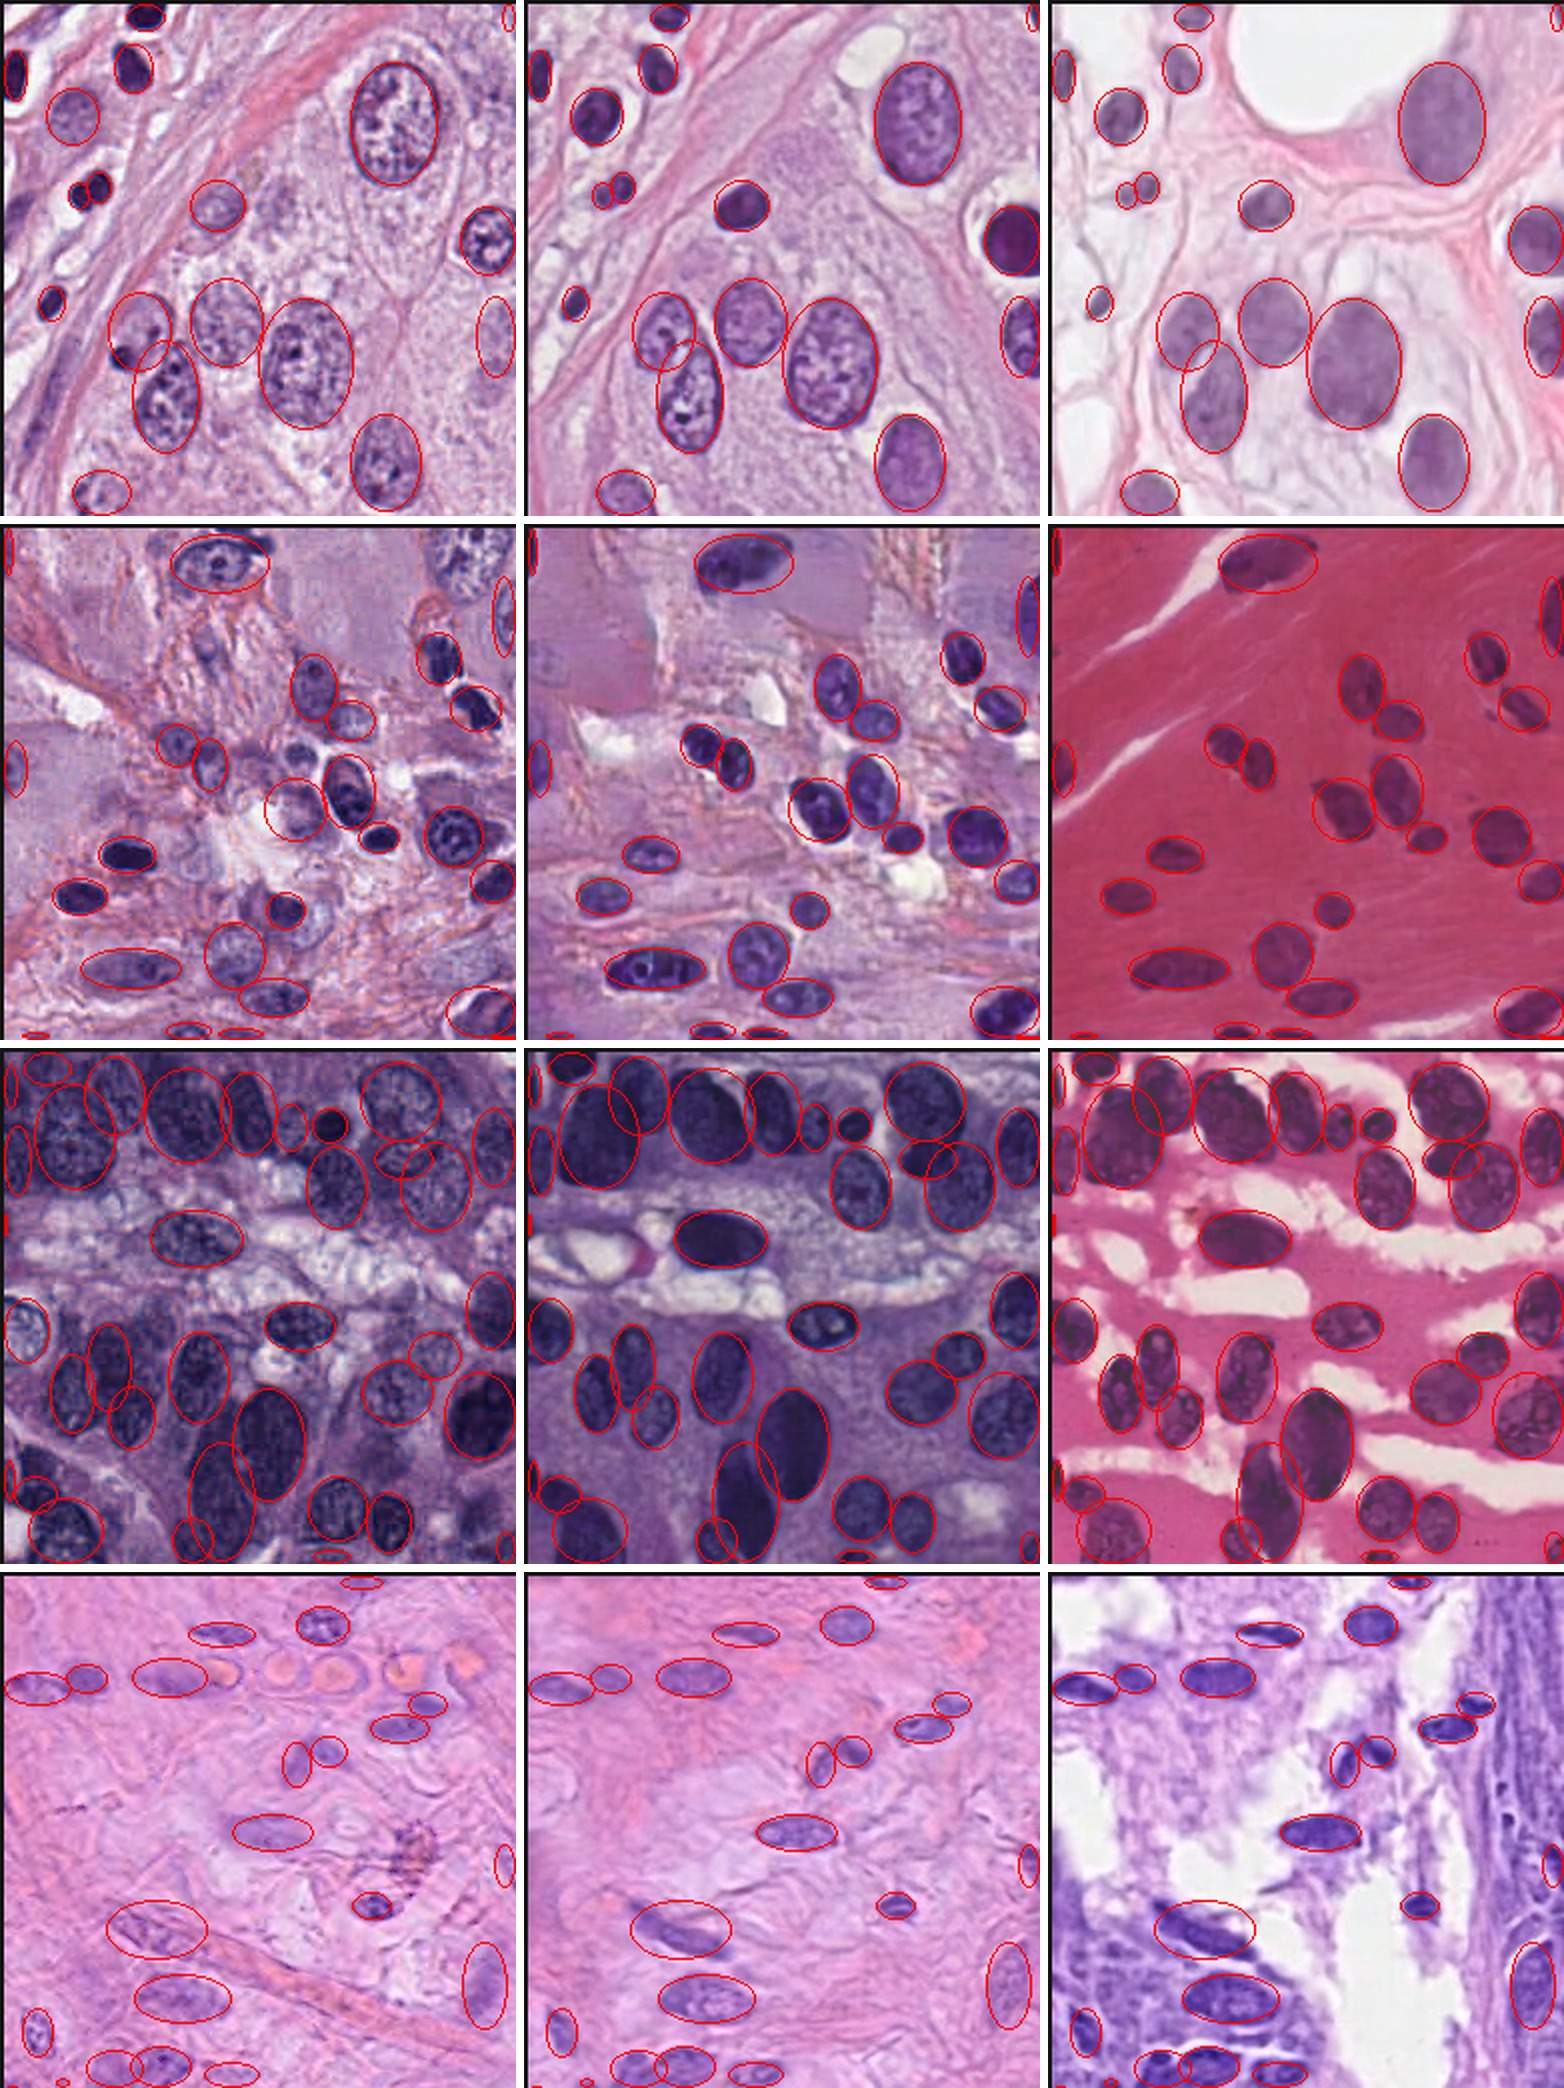
\includegraphics[width=0.7\linewidth]{figs/cf_arms.jpg}
\caption{同一张考卷图在“换背景/换染色”干预下重新生成的样子：红色轮廓是固定不变的标准答
案，细胞位置不变，画风变了。}
\label{fig:cfarms}
\end{figure}

原因有两层。第一，模型之间的真实差距主要在“找细胞”的能力上，而这种考试里“细胞位置不
变”，恰恰考不了“找细胞”；第二，它实际考的是“换了个背景还认不认得出类型”——而这几种模
型的两项能力恰好此消彼长，于是按后者排名，正好把前者的名次倒了过来。结论：这种考试只能
用来考“认类型”，不能当作跨病种能力的替身。

\section*{这份工作留下了什么}

\begin{itemize}
\item \textbf{一个明确的诊断}：凋亡核识别是检测问题。下一步最值得试的是让“找细胞”的部件
      在更高分辨率上工作（例如用更高分辨率的特征图来判断前景）——这是正式报告指出的开放
      方向，尚未验证。
\item \textbf{一份避坑指南}：评估 AI 时，别被单次实验的涨分骗到——先标定噪声有多大（见
      上）；看公开排行榜时留心评测配方的“水分”：有的已发布配方会在测试集上调参数——相当
      于考前对过答案——加上特殊技巧能白捡约 2 个百分点，比排行榜上多数名次差距还大；用
      生成数据做考试之前，先想清楚它到底考的是什么。
\item \textbf{可复现}：整套代码、数据管线与实验记录都保存在项目仓库里，每个结论都能逐步
      复现。
\end{itemize}

\vspace{1.5em}
\noindent\rule{\linewidth}{0.4pt}

\vspace{0.5em}
\noindent{\small 本文是《阶段报告一》的导读；完整的数字、表格与文献见同目录下的正式
报告（中文版 \texttt{stage\_report\_1\_zh.pdf}，英文版 \texttt{stage\_report\_1.pdf}）。}

\end{document}
